\section{Numerical Example}
\begin{figure}
	\centering
	\begin{subfigure}[t]{0.475\columnwidth}
		\centering
		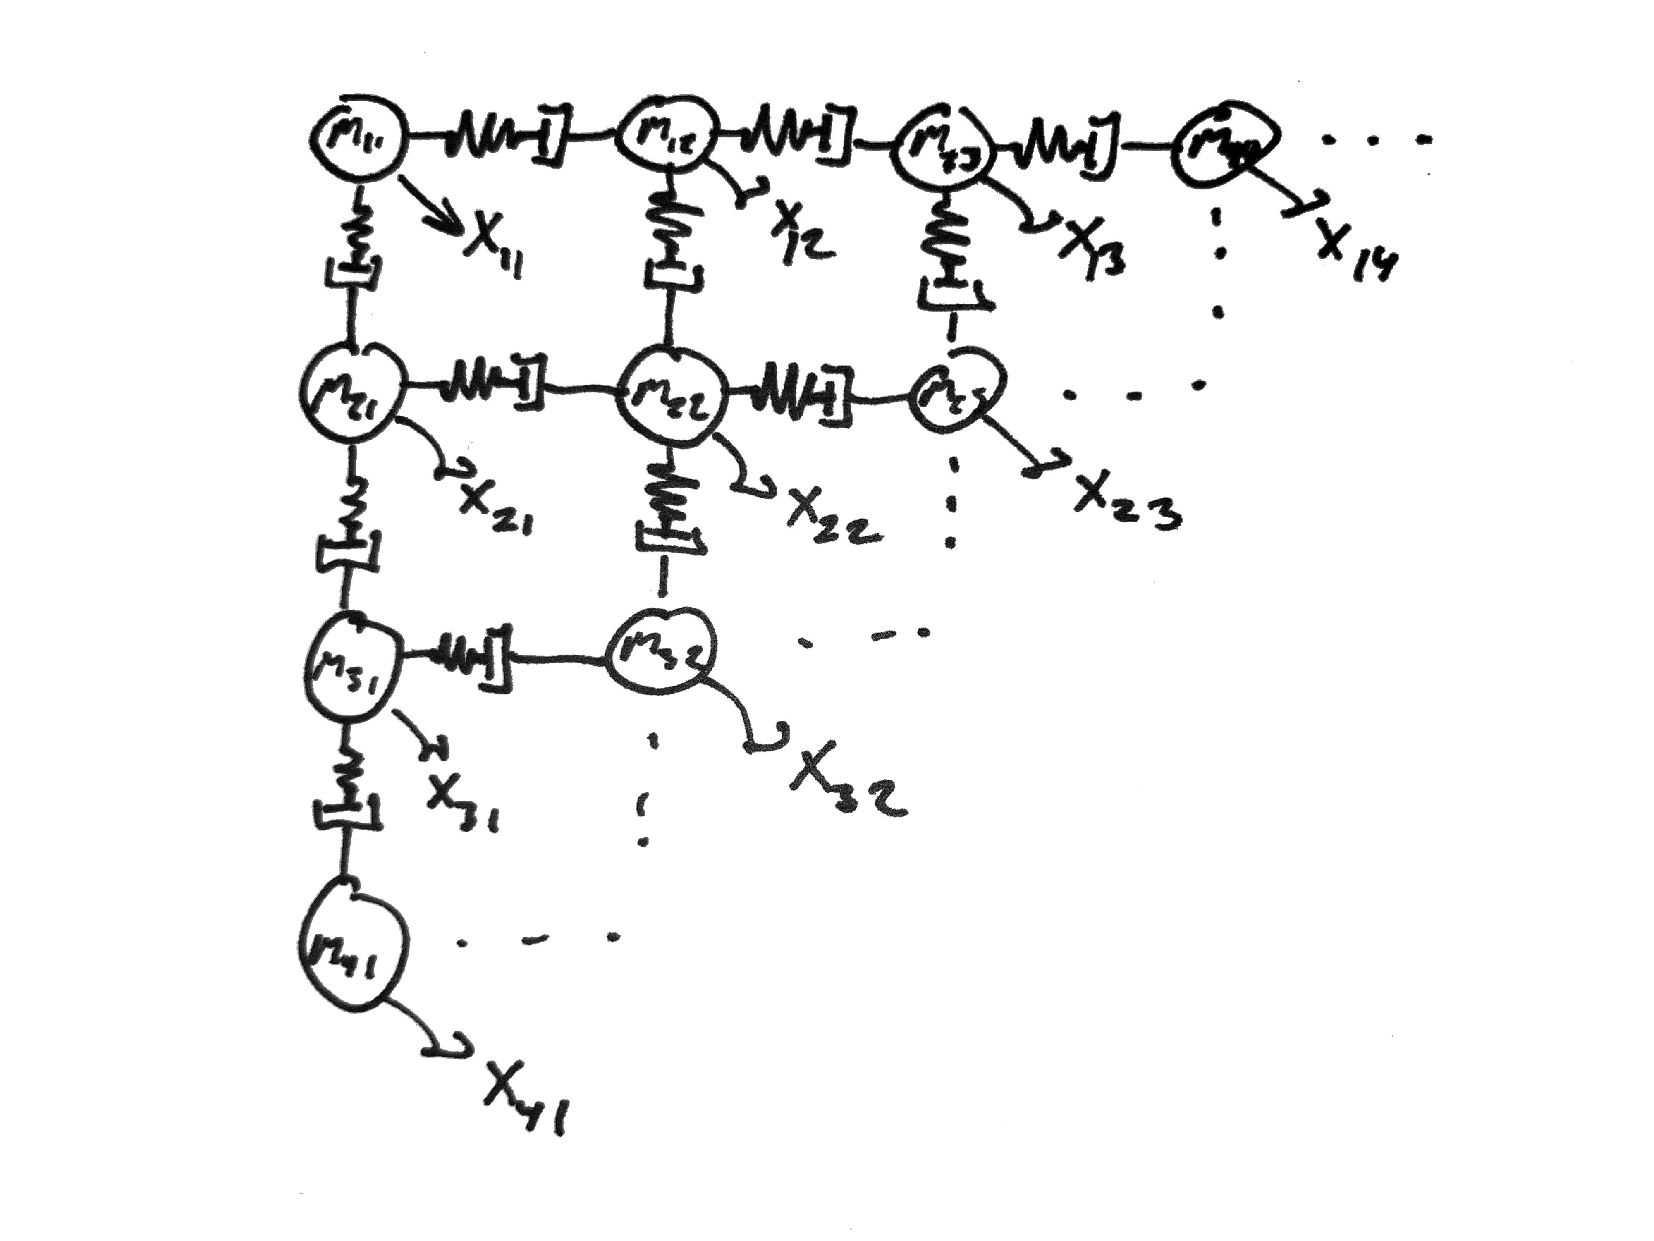
\includegraphics[width=\textwidth]{./figures/num_ex_sys}
		\caption{Array of linked spring-mass-damper systems. The mass of each object can switch independently according to a directed graph.}
		\label{fig:num_ex_sys}
	\end{subfigure}
	\hfill
	\begin{subfigure}[t]{0.475\columnwidth}
		\centering
		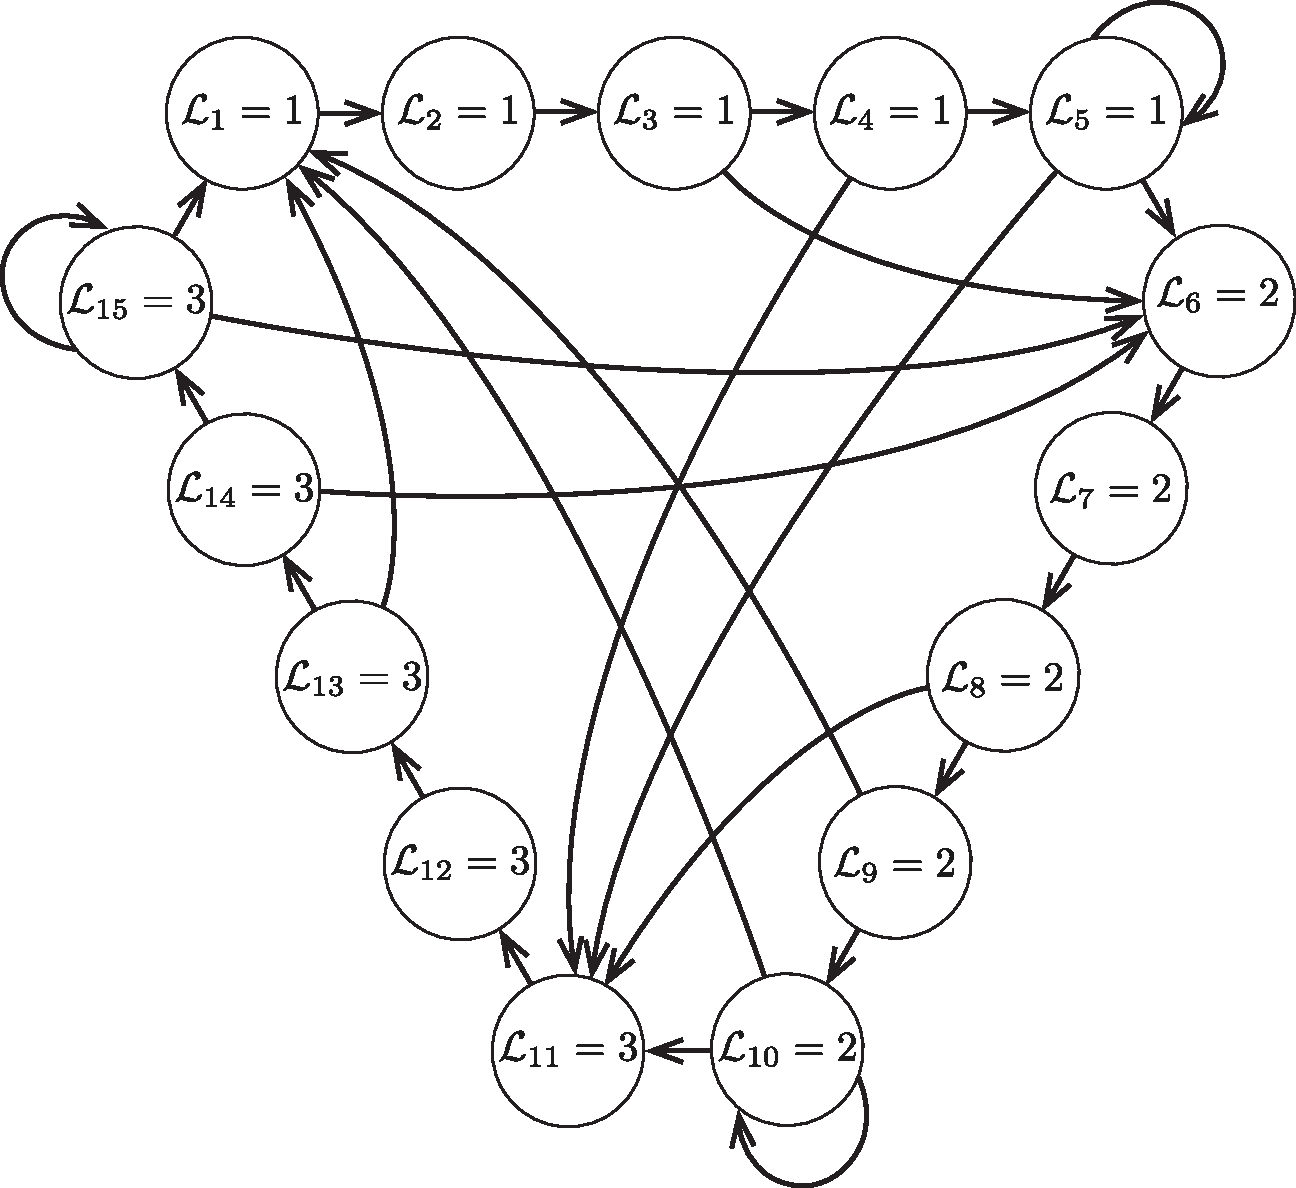
\includegraphics[width=\textwidth]{./figures/num_ex_graph}
		\caption{Directed graph controlling the switches of the numerical example. Note that the switching constraints cannot be encoded with minimum and maximum dwell times and demonstrate the flexibility of the proposed approach.}
		\label{fig:num_ex_graph}
	\end{subfigure}
	\caption{Description of the system used on the numerical example.}
\end{figure}

\begin{figure}[t]
\centering
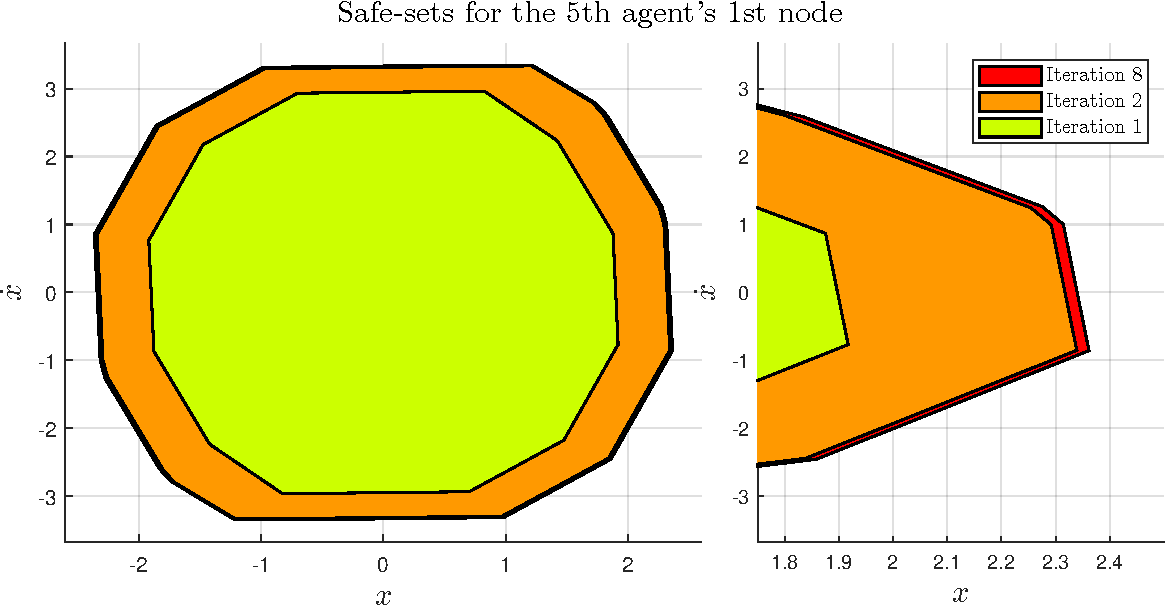
\includegraphics[width=\columnwidth]{./figures/num_ex_results}
\caption{Evolution of the safe-set for a single node of a single agent in the spring-mass-damper array. Though each safe-set shown is feasible, they monotonically increase to convergence with the number of iterations.}
\label{fig:num_ex_results}
\end{figure}

The results of this work are demonstrated in an array of independently controlled agents coupled with with springs and dampers as shown in \autoref{fig:num_ex_sys}. The objects move in the dimension denoted by $x_{i,j}$. The mass of each agent can switch between one of three values according to the directed graph shown in \autoref{fig:num_ex_graph}. For a system comprised of an $r\times c$ array of linked spring-mass-damper systems, the full state space will be in $\real^{2rc}$. Even for small, $2\times 2$ systems, the resulting 8D system is too large for previous set based methods. However, using the results of this work to parallelize the algorithm, only set operations in $\real^2$ are required. Assuming each agent has it's own independent processing, the computational complexity will grow at a sub-exponential rate with the number of agents. Running \autoref{alg:safe_sets} on the spring-mass-damper grid with randomized masses and spring/damper coefficients resulted in the safe-set evolution show in \autoref{fig:num_ex_results} for mode 1 of node 1. The numerical example implementation has been archived for future reference \alert{cite}. 